\section{Určitý integrál}
\begin{pozn}
    Supremum a infimum množiny jsme již zavedli v definici \ref{supinf}.
\end{pozn}

\begin{definition}
\textbf{Dělením} $D$ uzavřeného \textbf{intervalu} $\left < a,b \right > $
rozumíme každou konečnou množinu čísel $x_0,\dots,x_n \in \mathbb R$ takových, že
$a=x_0<x_1<\dots<x_n=b.$ Intervaly $\left < x_0, x_1 \right >$,
$\left < x_1, x_2 \right >$, $\dots$, $\left < x_{n-1}, x_n \right >$ nazýváme
\textbf{dělící intervaly}, které označíme $D=\left \{ x_0,x_1,\dots,x_n \right \} .$
Body $x_0,\dots,x_n$ nazýváme \textbf{dělící body} dělení $D$. Číslo
$\max \left ( x_i-x_{i-1} \right ), i=1,\dots,n $ nazýváme \textbf{normou dělení}
$D$ a označujeme $\nu(D).$ Množinu všech dělení na intervalu $\left < a,b \right > $
označme $\mathscr D(a,b).$
\end{definition}

\begin{figure}[ht!]
  \centering
  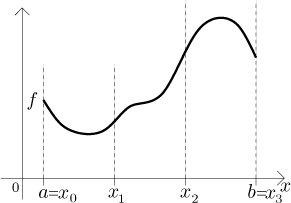
\includegraphics[width=0.32\textwidth]{images/deleni.png}
  \caption{Dělení $D=\left \{ x_0, x_1, x_2, x_3 \right\}$.}
\end{figure}

\begin{definition}
Nechť $D_1, D_2 \in \mathscr D(a,b)$. Řekneme, že dělení $D_2$ je \textbf{zjemněním
dělení} $D_1,$ jestliže $D_1 \subset D_2.$
\end{definition}

\begin{definition}
Nechť $f(x)$ je omezená na $\left < a,b \right > , D\in \mathscr D(a,b),
D=\left \{ x_0,\dots,x_n \right \}. $ Pak množina $\left \{ f(x),
x \in \left < x_{i-1},x_i \right >  \right \} $ je pro všechna $i \in \left \{
1,\dots,n\right \} $ neprázdná a omezená a tedy má supremum a infimum.
Označme
\begin{align*}
    m_i &= \inf \left \{ f(x), x \in \left < x_{i-1},x_i \right >  \right \} \textrm{ pro } D=\left \{ x_0,\dots,x_n \right \},\\
    M_i &=   \sup \left \{ f(x), x \in \left < x_{i-1},x_i \right >  \right \} \textrm{ pro } D=\left \{ x_0,\dots,x_n \right \}.
\end{align*}
Číslo $S(D,f)=\sum_{i=1}^n M_i\cdot (x_i-x_{i-1})$
(resp. $s(D,f)=\sum_{i=1}^n m_i\cdot (x_i-x_{i-1})$) je \textbf{horní} (resp. \textbf{dolní}) \textbf{součet funkce}
$f(x)$ příslušný dělení $D$.
\end{definition}

\begin{figure}[ht!]
  \centering
  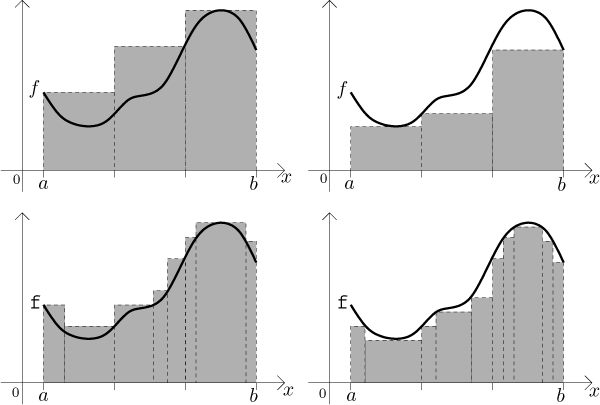
\includegraphics[width=0.6\textwidth]{images/riemannuv_int.png}
  \caption{Horní (vlevo) a dolní (vpravo) součty funkce $f(x)$.}
\end{figure}

\begin{pozn}
    Platí $s(D,f)\leq S(D,f).$
\end{pozn}

\begin{veta}
Nechť $f(x)$ je omezená na intervalu $\left < a,b \right >. $ Pak
$\left \{ s(D,f); D\in \mathscr D(a,b) \right \} $ je shora omezená a množina
$\left \{ S(D,f); D\in \mathscr D(a,b) \right \} $ je zdola omezená.
\end{veta}

\begin{pozn}
     Množina dolních součtů má supremum a množina horních součtů má infimum.
\end{pozn}

\begin{definition}
Nechť $f(x)$ je omezená na intervalu $\left < a,b \right > .$ Označme
\begin{align*}
    \int_{\underline{a}} ^b f(x) \, dx & = \sup \left \{ s(D,f); D \in \mathscr D(a,b) \right \}, \\
    \int_{a} ^{\underline{b}} f(x) \, dx & = \inf \left \{ S(D,f); D \in \mathscr D(a,b) \right \}.
\end{align*}
Číslo $\int_{\underline{a}} ^b f(x)\, dx$ (resp. $\int_{a} ^{\underline{b}} f(x) \, dx$)
nazýváme \textbf{dolní} (resp. \textbf{horní}) \textbf{integrál} funkce $f(x)$ od
$a$ do $b$.
\end{definition}

\begin{veta}
Nechť $f(x)$ je omezená na intervalu $\left < a,b \right >. $ Pak
$$\int_{\underline{a}} ^b f(x)\, dx \leq \int_{a} ^{\underline{b}} f(x) \, dx.$$
\end{veta}

\begin{definition}
Nechť $f(x)$ je omezená na intervalu $\left < a,b \right > .$ Pak funkce
$f(x)$ je na intervalu $\left < a,b \right > $ (Riemmanovsky) \textbf{integrovatelná}
(integrace schopna), jestliže
$$\int_{\underline{a}} ^b f(x)\, dx = \int_{a} ^{\underline{b}} f(x) \, dx.$$
Je-li $f(x)$ na intervalu $\left < a,b \right > $ integrovatelná, klademe
$$\int_{\underline{a}} ^b f(x)\, dx = \int_{a} ^{\underline{b}} f(x) \, dx = \int_{a} ^b f(x) \, dx.$$
Číslo $\int_{a} ^b f(x)\, dx$ nazýváme \textbf{Riemannův integrál} funkce $f(x)$ od
$a$ do $b$. Pokud $\int_{\underline{a}} ^b f(x)\, dx < \int_{a} ^{\underline{b}} f(x) \, dx$,
pak $f(x)$ není na intervalu $\left < a,b \right > $ integrovatelná a
$\int_{a} ^b f(x)\, dx$ nedefinujeme.
\end{definition}

\begin{veta}[Newton-Leibnitzova věta]
Nechť $f(x)$ je integrovatelná na intervalu $\left < a,b \right >$, $F(x)$ je spojitá
na intervalu $\left < a,b \right > $. Buď $F(x)$ primitivní funkce k funkci $f(x)$
na intervalu $\left ( a,b \right ) $. Pak platí:
$$\int_{a} ^b f(x)\, dx=F(b)-F(a).$$
\end{veta}

\begin{veta}
Nechť $f(x)$ je spojitá na intervalu $\left < a,b \right > $. Pak $f(x)$ je na
intervalu $\left < a,b \right > $ integrovatelná.
\end{veta}

\begin{priklad}
Vypočtěte integrál $\int_0^{\frac{\pi}{4}}\cos x \, dx.$
\end{priklad}

\begin{reseni}
Platí
$$\int_0^{\frac{\pi}{4}}\cos x \, dx=\left [ \sin x  \right ]_0^{\frac{\pi}{4}}=\sin \frac{\pi}{4}-\sin 0=\frac{\sqrt{2} }{2}. $$
\end{reseni}

\begin{veta}
Nechť $f(x), f_1(x),\dots,f_n(x), g(x)$ jsou integrovatelné funkce na intervalu $\left < a,b \right > $
a~$c; c_1,\dots,c\in \mathbb R.$ Pak
\begin{enumerate}[$i.$]
\item funkce $f(x)+g(x)$ je integrovatelná na int. $\left < a,b \right > $ a platí
$$\int _a^b \left [ f(x)+g(x) \right ] \, dx = \int_a ^b f(x)\, dx + \int_a ^b g(x) \, dx,$$
\item funkce $c\cdot f(x)$ je integrovatelná na int. $\left < a,b \right > $ a platí
$$\int _a ^b c\cdot f(x) \, dx = c \int _a ^b f(x)\, dx,$$
\item funkce $c_1\cdot f_1(x) + \dots + c_n \cdot f_n(x)$ je integrovatelná na int. $\left < a,b \right > $ a platí
$$\int_a ^b \left [ c_1\cdot f_1(x) + \dots + c_n \cdot f_n (x) \right ]\, dx = c_1 \int _a ^b f_1(x)\, dx + \dots + c_n \int _a ^b f_n(x)\, dx. $$
\end{enumerate}
\end{veta}

\begin{veta}
Nechť $f(x)$ je integrovatelná a nezáporná na intervalu $\left < a,b \right > $. Pak
$$\int_a ^b f(x) \, dx \geq 0.$$
\end{veta}

\begin{veta}
Nechť funkce $f(x),g(x)$ jsou integrovatelné na intervalu $\left < a,b \right > .$
Nechť pro každé $x\in \left < a,b \right > :f(x)\leq g(x).$ Pak
$$\int_a^b f(x) \, dx \leq \int_a^b g(x) \, dx.$$
\end{veta}

\begin{veta}
Nechť $a<b<c$ jsou reálná čísla a $f(x)$ je integrovatelná na intervalech
$\left < a,b \right >$, $\left < b,c \right >$. Pak
$$\int_a^c f(x)\, dx = \int_a^b f(x)\, dx + \int_b^c f(x)\, dx.$$
\end{veta}

\begin{definition}\label{pocastechspoj}
Funkce $f(x)$ se nazývá \textbf{po částech spojitá} na intervalu $\left < a,b \right > $,
jestliže je na intervalu $\left < a,b \right > $ spojitá s výjimkou konečného počtu
bodů $c_1,\dots,c_n; a<c_1<\dots<c_n<b.$
\end{definition}

\begin{veta}
Nechť funkce $f(x)$ je po částech spojitá na intervalu $\left < a,b \right > $, jako
v definici \ref{pocastechspoj}. Pak
$$\int_a^b f(x)\, dx = \int_a^{c_1}f(x)\, dx + \int_{c_1}^{c_2}f(x)\, dx + \dots + \int_{c_n}^b f(x)\, dx.$$
\end{veta}

\begin{definition}
Je-li $f(x)$ definována v čísle $a \in \mathbb R,$ klademe
$$\int _a ^a f(x)\, dx = 0.$$
Je-li $f(x)$ integrovatelná na intervalu $\left < a,b \right >$, definujeme
$$\int_b^a f(x)\, dx = -\int_a^b f(x)\, dx.$$
\end{definition}


\begin{veta}[O substituci pro určité integrály]\label{ppui}
Nechť $\varphi (t)$, $\varphi: \left < \alpha, \beta \right >\to \left < a,b \right >  $ má na intervalu $\left < \alpha, \beta  \right > $ spojitou derivaci
$\varphi^\prime (t)$ a~nechť $f(x)$ je spojitá na intervalu $\left < a,b \right >$.
Označme
$\varphi(\alpha)=a, \varphi(\beta)=b.$ Pak platí
$$\int _a ^b f(x)\, dx = \int _\alpha ^\beta f \left [ \varphi(t) \right ]\cdot \varphi^\prime (t)\, dt. $$
\end{veta}

\begin{pozn}
    Ve větě \ref{ppui} využíváme tzv. \textbf{transformace mezí}.
\end{pozn}

\begin{priklad}
Vypočtěte integrál $\int _1^2 \frac{x}{(1+x^2)}\, dx.$
\end{priklad}

\begin{reseni}
Musíme provést transformaci mezí:
\begin{align*}
\int _1^2 \frac{x}{(1+x^2)}\, dx &= \left |\begin{array}{l l}
    t=x^2+1 & x=2\implies t=5 \\
    dt = 2x \, dx & x=1\implies t=2
\end{array}\right | = \frac{1}{2}\int _2^5 \frac{1}{t^{\frac{3}{2}}}\, dt \\
&= \frac{1}{2}\left [ \frac{t^{-\frac{1}{2}}}{-\frac{1}{2}} \right ] _2^5 = \frac{1}{2}\left ( \frac{5^{-\frac{1}{2}}}{-\frac{1}{2}}-\frac{2^{-\frac{1}{2}}}{-\frac{1}{2}} \right )=-\frac{1}{\sqrt{5} }+\frac{1}{\sqrt{2} }.
\end{align*}
\end{reseni}

\begin{veta}[O integraci \textit{per partes} pro určité integrály]
Nechť funkce $u(x)$ a $v(x)$ mají na intervalu $\left < a,b \right > $ spojité derivace
$u^\prime (x)$ a $v^\prime (x)$. Pak platí
$$\int_a ^b u^\prime (x)v(x)\, dx = \left [ u(x)v(x) \right ]_a^b -\int _a^b u(x)v^\prime(x)\,dx.$$
\end{veta}

\begin{priklad}
Vypočtěte integrál $\int _0^{\frac{\pi}{2}}x \cos \frac{x}{2}\, dx$.
\end{priklad}

\begin{reseni}
Platí
\begin{align*}
\int _0^{\frac{\pi}{2}}x \cos \frac{x}{2}\, dx &= \left | \begin{array}{ll}
    u=x & u^\prime = 1 \\
    v^\prime = \cos \frac{x}{2} & v = 2\sin \frac{x}{2}
\end{array}   \right | \\
& =\left [ x\cdot2\sin \frac{x}{2} \right ]_0^{\frac{\pi}{2}}-\int_0^{\frac{\pi}{2}}2\sin \frac{x}{2}\, dx =\frac{\pi}{2}\cdot \frac{\sqrt{2} }{2}-0-\left [ -4\cos \frac{x}{2} \right ]_0^{\frac{\pi}{2}}\\
&= \pi \cdot \frac{\sqrt{2} }{2}+4\cdot \frac{\sqrt{2} }{2}-4
\end{align*}
\end{reseni}

\begin{pozn}
    Je-li $f(x)$ spojitá a nezáporná na intervalu $\left < a,b \right >$, je
    $\int_a ^b f(x)\, dx$ obsah plochy omezené osou $x$, přímkami $x=a, x=b$ a
    grafem funkce $y=f(x)$. Platí tedy
    $$S=\int_a^b f(x)\, dx.$$
\end{pozn}

\begin{priklad}
Vypočtěte obsah plochy $M=\left \{ [x,y]; y \geq  x^2 , y \leq 2x\right \} $.
\end{priklad}

\begin{reseni}
Nejprve určíme průsečíky funkcí $x^2$ a $2x$: $x_1=0,x_2=2$. Plochu spočítáme
jako
$$\int_0^2 2x\, dx - \int_0^2 x^2 \, dx.$$
\end{reseni}

\begin{priklad}
Vypočtěte obsah kruhu o poloměru $r$.
\end{priklad}

\begin{reseni}
Počítáme $2\int_{-r}^r \sqrt{r^2-x^2}\, dx  $.
\end{reseni}

\begin{pozn}
    Nechť je $f(x)$ spojitá a nezáporná na intervalu $\left < a,b \right >$ a je
    dána množina bodů
    $M=\left \{ \left [ x,y \right ]; x \in \left < a,b \right >,\linebreak y \in \left < y, f(x) \right >    \right \} .$
    Nechť $M$ rotuje kolem osy $x$. Dostaneme rotační těleso, jehož objem je
    $$V=\pi \int _a^b \left [ f(x) \right ]^2 \, dx. $$
\end{pozn}

\begin{priklad}
Vypočtěte objem koule o poloměru $r$.
\end{priklad}

\begin{reseni}
Počítáme $\pi\int _{-r}^r(\sqrt{r^2-x^2} )^2 \, dx=\pi\int_{-r}^r(r^2-x^2)\, dx$.
\end{reseni}

\begin{pozn}
Nechť je $f(x)$ funkce se spojitou derivací na intervalu $\left < a,b \right > $. Délka
grafu funkce $f(x)$ je
$$L=\int_a^b \sqrt{1+(f^\prime(x))^2}\, dx. $$
\end{pozn}

\begin{priklad}
Spočtěte délku kružnice o poloměru $r$.
\end{priklad}

\begin{reseni}
Počítáme $2\int _{-r}^r \sqrt{1+\left ( \frac{-x}{\sqrt{r^2-x^2}} \right )^2 }\, dx.  $
\end{reseni}

\begin{pozn}
    Nechť $f(x)$ je funkce se spojitou derivací na intervalu $\left < a,b \right > .$
    Pak plášť rotačního kužele, který vznikne rotací grafu $f(x)$ kolem osy $x$, má
   povrch
  $$S=2\pi\int_a^b f(x)\cdot \sqrt{1+(f^\prime(x))^2}\, dx. $$
\end{pozn}

\begin{priklad}
Určete povrch koule o poloměru $r$.
\end{priklad}

\begin{reseni}
Počítáme $S=2\pi\int_{-r}^r \sqrt{r^2-x^2}\cdot \sqrt{1+\left ( \frac{-x}{\sqrt{r^2-x^2} } \right )^2 } \, dx. $
\end{reseni}
